\documentclass[12pt,a4paper]{report}
\usepackage[latin1]{inputenc}
\usepackage{amsmath}
\usepackage{amsfonts}
\usepackage{subfigure}
\usepackage{amssymb}
\usepackage[pdftex]{graphicx}
\begin{document}

\noindent
{\bf Part I: Convolutional Sparse Coding} \\ \\
A baseline dictionary consisting of 16 convolution kernels was obtained using Sparse Coding with FISTA inference.
\begin{itemize}
\item These experiments were run on contrast normalized color CIFAR-10.  
\item All experiments used a constant learning rate (different for each experiment), sparsity weight of $\alpha = 0.5$, and mini-batches of 16. 
\item Each kernel in the dictionary was re-normalized to unit $L_2$-norm after every update.   
\end{itemize}  
Here are the filters I obtained:
\begin{center}

\includegraphics[scale=4]{dec_SC1.png}
\end{center} 
After the dictionary was trained, the optimal sparse codes were inferred with FISTA using the same termination criterion as was used during training. Convergence was assumed when $L_2$ change in codes between iterations was less than 5\%.   
These codes produced an average per-pixel loss of: 
\begin{equation}
L_{FISTA} = \min_Z \frac{1}{2}\|X-W_dZ\| + \alpha |Z|_1 \approx 0.02476
\end{equation} 
Here is a sample of 16 input images: 

\begin{figure}[ht]
	\begin{center}
	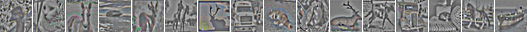
\includegraphics[scale=0.75]{sample.png}
	
\includegraphics[scale=0.75]{rec.png}
	\caption{Sample input images (top), Reconstructions (bottom)} 
	\end{center}
\end{figure} 

Figure 2 shows the activations inferred via FISTA for this dictionary on the sample images. The first row, corresponds to the first image (the ostrich), etc. Each row shows the activations for all 16 filters. The activations are quite sparse (5.3\% of the activations are non-zero over the entire dataset), and intuitive. 
\begin{figure}[ht]
	\begin{center}
	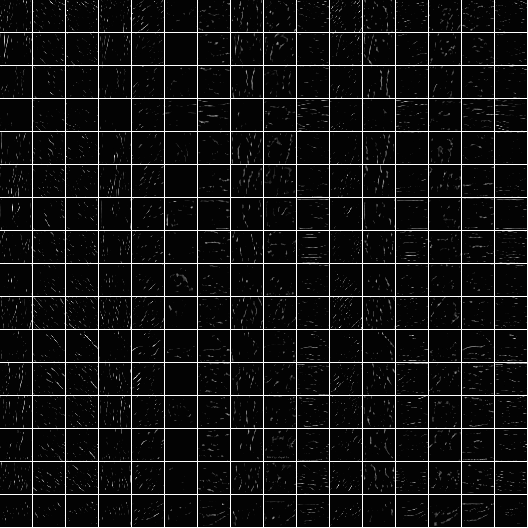
\includegraphics[scale=0.75]{target.png}
	\end{center}
	\caption{Feature maps for all 16 filters for the 16 sample images. Each row corresponds to the same input image, each column corresponds to the same filter.}
\end{figure} 
\newpage
{\bf Part II: LISTA Sanity Check} \\ \\
Since adding more LISTA loops corresponds to doing more ISTA iterations, a good sanity check of the LISTA network is to check weather the two are indeed equivalent. 
I did this in two ways: 
\begin{itemize} 
\item {(i) checked that add adding more LISTA loops indeed lowers the inference cost (Equation 1). Here are some typical (unnormalized) losses as function of the number of loops for a random decoder and random input:\\ \\
$L_0 = 761.48$\\
$L_1 = 729.10$\\
$L_5 = 369.54$}
\item{Next, I compared the loss corresponding to $n$-steps of ISTA and the loss corresponding to the code produced by fprop of an $n-1$-loop LISTA network. Here are some values for 3-ISTA iterations: \\ \\
$L_{ISTA} = 0.15376$\\
$L_{LISTA} = 0.15342$} \\ \\ I believe the discrepancy is caused by numerical issues stemming from the differences in implementation of ISTA and LISTA (i.e. ISTA uses only $W_d$, LISTA also uses $S$). 
\end{itemize} 
 

{\bf Part III: Training Convolutional LISTA Inference} \\ \\
I trained a LISTA encoders with varying number of loops ($LISTA_n$ corresponds to a LISTA network with $n$-loops) in two experiments: 
\begin{itemize} 
\item Experiment 1: regress directly on the codes (as in Karol's paper): 
\begin{equation} 
\nonumber 
\min_{W_e,S} \|Z_{FISTA} - LISTA_n(X;W_e,S) \|
\end{equation}  
\item Experiment 2: minimize the loss, with a fixed, normalized decoder: 
\begin{equation} 
\nonumber
\min_{W_e,S} \frac{1}{2} \|X - W_d Z\| + \alpha |Z|_1 ~ \mbox{where}~ Z = LISTA_n(X;W_e,S)
\end{equation}
\end{itemize} 

In both experiments, increasing the number of loops helps reduce the code-prediction error or loss.  
\begin{figure}
	\begin{center}
	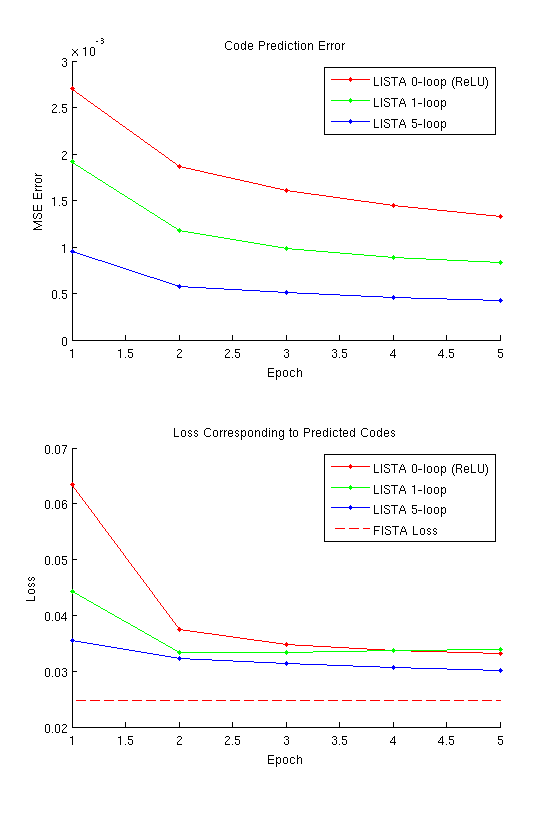
\includegraphics[scale=0.75]{code_pred.png}
	\end{center}
\caption{Results for Experiment 1}
\end{figure} 
\begin{figure}
	\begin{center}
	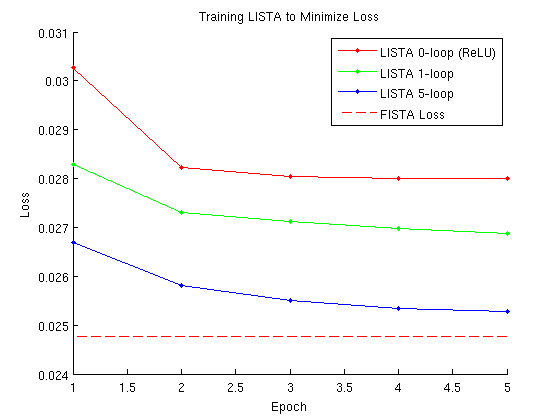
\includegraphics[scale=0.75]{LISTA_loss_min.png}
	\end{center}
\caption{Results for Experiment 2}
\end{figure} 

{\bf Part IV: Auto-Encoder Dictionary Learning using LISTA } \\ \\
In this setting, we are interested in minimizing:  
\begin{equation} 
\min_{W_e,S,Wd} \frac{1}{2} \|X - W_d Z\| + \alpha |Z|_1 ~ \mbox{where}~ Z = LISTA_n(X;W_e,S)
\end{equation}
An auto-encoder will minimize this loss w.r.t. to $Z$ (parameterized by $W_e$ and $S$) and $W_d$ simultaneously usually via s.g.d. This is the same way that DrSAE (by Jason Rolf) uses LISTA. This is the same as Experiment 2 above, except we let the decoder learn as well. \\ \\
\textbf{Contrary to previous findings, I found that in this setting encoders with more than one LISTA loop \emph{do not} attain a lower loss.} \\ \\
\textbf{The auto-encoders converge much faster, and often find a better minimum than iterative sparse coding with FISTA inference (when run for the same number of iterations).} \\ \\
All the following models were trained with a constant learning rate (optimized for that model) for 100 epochs. The auto-encoders were trained with $\alpha=3$, sparse coding with $\alpha=0.5$, \textbf{but the loss for all models was evaluated with $\alpha=0.5$}.    

\begin{center}
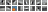
\includegraphics[scale=4]{dec_SC2.png}(1) \\
\vspace{0.5cm} 
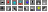
\includegraphics[scale=4]{LISTA1_dec.png}(2) \\
\vspace{0.5cm} 
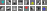
\includegraphics[scale=4]{LISTA2_dec.png}(3)
\end{center}
Top to bottom: bases found with (1) sparse coding, (2) LISTA auto-encoder with 1-loop, (3) LISTA auto-encoder with 2-loops. 
Here are the performance results for all three models. The reconstruction error is the per-pixel MSE error (~11.4\% for sparse coding). Percent $L_0$ is the percent of the activations which are greater than zero. The best model in every measure, is the 1-loop LISTA auto-encoder. 
\\ \\    
\texttt{ 
=====Sparse Coding===== \\
Percent Rec Error:0.11413859299469\\
Percent L0       :0.089237814941406\\
Loss             :0.024767283491965\\
=====LISTA1-Auto-Enc=====\\
Percent Rec Error:0.064871864133431\\
Percent L0       :0.087790825195313\\
Loss             :0.018787112789303\\
=====LISTA2-Auto-Enc=====\\
Percent Rec Error:0.062972138407044\\
Percent L0       :0.095947513427734\\
Loss             :0.01844597114861\\
}



\end{document}